\documentclass[tikz,border=10pt]{standalone}
\usepackage[T1]{fontenc}
\usepackage{helvet}
\renewcommand{\familydefault}{\sfdefault}
\usepackage{amsmath,amssymb}
\usepackage{tikz}
\usetikzlibrary{calc,positioning,fit,arrows.meta,shapes.geometric}

% Canonical Academic Palette
\definecolor{OxfordNavy}{HTML}{1E293B}
\definecolor{SlateSteel}{HTML}{334155}
\definecolor{MutedTeal}{HTML}{0F766E}
\definecolor{TealL0}{HTML}{F0FDFA}
\definecolor{Burgundy}{HTML}{991B1B}
\definecolor{BurgundyL0}{HTML}{FEF2F2}
\definecolor{WarmOchre}{HTML}{92400E}
\definecolor{OchreL0}{HTML}{FFFBEB}
\definecolor{ForestSage}{HTML}{166534}
\definecolor{SageL0}{HTML}{F0FDF4}
\definecolor{CoolParchment}{HTML}{F8FAFC}
\definecolor{SlateRim}{HTML}{CBD5E1}
\definecolor{GridGray}{HTML}{E2E8F0}
\definecolor{DarkSlate}{HTML}{0F172A}
\definecolor{Amethyst}{HTML}{6B21A8}
\definecolor{AmethystL0}{HTML}{FAF5FF}

\begin{document}
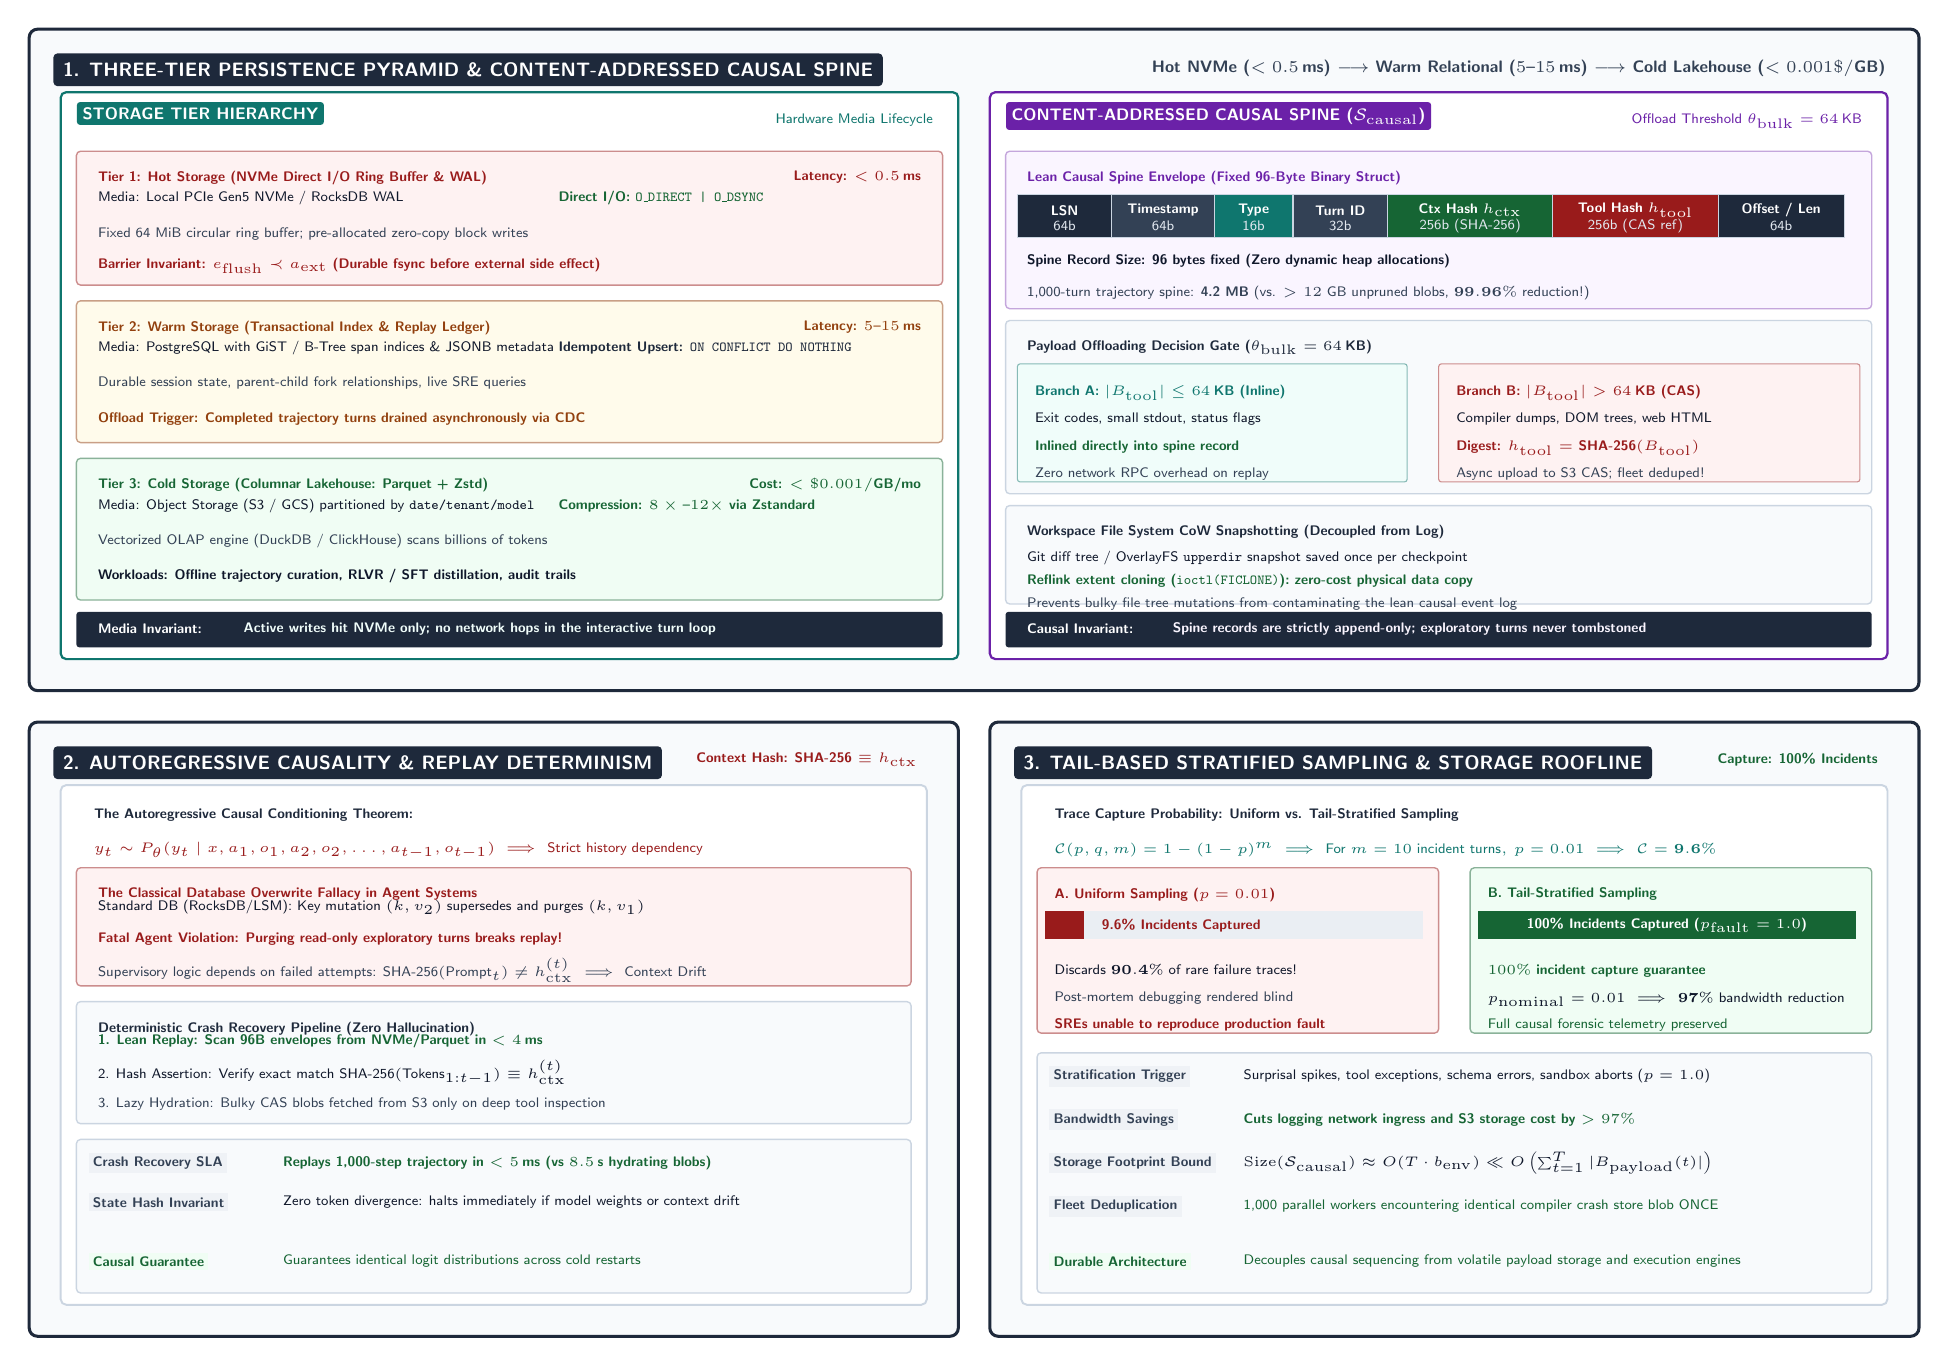
\begin{tikzpicture}[
  font=\sffamily,
  scale=1.0,
  >=Stealth,
  node distance=0.5cm
]

% =============================================================================
% TOP TIER: THREE-TIER PERSISTENCE PYRAMID & CAUSAL SPINE (y: 8.2 to 16.6)
% =============================================================================
\begin{scope}[shift={(0, 8.2)}]
  \draw[fill=CoolParchment, draw=OxfordNavy, line width=1.1pt, rounded corners=3pt]
    (0, 0) rectangle (24.0, 8.4);

  % Top Headers
  \node[anchor=north west, fill=OxfordNavy, text=white, font=\fontsize{7.5}{9.0}\selectfont\bfseries, rounded corners=1.5pt, inner sep=3.5pt]
    at (0.3, 8.1) {1. THREE-TIER PERSISTENCE PYRAMID \& CONTENT-ADDRESSED CAUSAL SPINE};
  \node[anchor=east, text=SlateSteel, font=\fontsize{6.0}{7.2}\selectfont\bfseries]
    at (23.7, 7.9) {Hot NVMe ($<0.5\,\text{ms}$) $\longrightarrow$ Warm Relational ($5\text{--}15\,\text{ms}$) $\longrightarrow$ Cold Lakehouse ($<0.001\$/\text{GB}$)};

  % --- LEFT COLUMN: 3-TIER HARDWARE STORAGE LIFECYCLE (x: 0.4 to 12.0) ---
  \begin{scope}[shift={(0.4, 0.4)}]
    \draw[fill=white, draw=MutedTeal, line width=0.8pt, rounded corners=2pt] (0, 0) rectangle (11.4, 7.2);

    \node[anchor=north west, fill=MutedTeal, text=white, font=\fontsize{5.8}{6.8}\selectfont\bfseries, rounded corners=1pt, inner sep=2pt]
      at (0.2, 7.08) {STORAGE TIER HIERARCHY};
    \node[anchor=north east, font=\fontsize{4.6}{5.4}\selectfont, text=MutedTeal]
      at (11.2, 7.05) {Hardware Media Lifecycle};

    % Tier 1: Hot Tier Box
    \draw[fill=BurgundyL0, draw=Burgundy!50, line width=0.5pt, rounded corners=1.5pt] (0.2, 4.75) rectangle (11.2, 6.45);
    \node[anchor=north west, font=\fontsize{5.0}{6.0}\selectfont\bfseries, text=Burgundy] at (0.35, 6.32) {Tier 1: Hot Storage (NVMe Direct I/O Ring Buffer \& WAL)};
    \node[anchor=north east, font=\fontsize{4.5}{5.2}\selectfont\bfseries, text=Burgundy] at (11.05, 6.32) {Latency: $< 0.5\,\text{ms}$};

    \node[anchor=west, font=\fontsize{4.4}{5.2}\selectfont, text=DarkSlate] at (0.35, 5.85) {Media: Local PCIe Gen5 NVMe / RocksDB WAL};
    \node[anchor=west, font=\fontsize{4.4}{5.2}\selectfont\bfseries, text=ForestSage] at (6.2, 5.85) {Direct I/O: \texttt{O\_DIRECT | O\_DSYNC}};
    \node[anchor=west, font=\fontsize{4.3}{5.1}\selectfont, text=SlateSteel] at (0.35, 5.40) {Fixed 64 MiB circular ring buffer; pre-allocated zero-copy block writes};
    \node[anchor=west, font=\fontsize{4.3}{5.1}\selectfont\bfseries, text=Burgundy] at (0.35, 5.00) {Barrier Invariant: $e_{\mathrm{flush}} \prec a_{\mathrm{ext}}$ (Durable fsync before external side effect)};

    % Tier 2: Warm Tier Box
    \draw[fill=OchreL0, draw=WarmOchre!50, line width=0.5pt, rounded corners=1.5pt] (0.2, 2.75) rectangle (11.2, 4.55);
    \node[anchor=north west, font=\fontsize{5.0}{6.0}\selectfont\bfseries, text=WarmOchre] at (0.35, 4.42) {Tier 2: Warm Storage (Transactional Index \& Replay Ledger)};
    \node[anchor=north east, font=\fontsize{4.5}{5.2}\selectfont\bfseries, text=WarmOchre] at (11.05, 4.42) {Latency: $5\text{--}15\,\text{ms}$};

    \node[anchor=west, font=\fontsize{4.4}{5.2}\selectfont, text=DarkSlate] at (0.35, 3.95) {Media: PostgreSQL with GiST / B-Tree span indices \& JSONB metadata};
    \node[anchor=west, font=\fontsize{4.4}{5.2}\selectfont\bfseries, text=OxfordNavy] at (6.2, 3.95) {Idempotent Upsert: \texttt{ON CONFLICT DO NOTHING}};
    \node[anchor=west, font=\fontsize{4.3}{5.1}\selectfont, text=SlateSteel] at (0.35, 3.50) {Durable session state, parent-child fork relationships, live SRE queries};
    \node[anchor=west, font=\fontsize{4.3}{5.1}\selectfont\bfseries, text=WarmOchre] at (0.35, 3.05) {Offload Trigger: Completed trajectory turns drained asynchronously via CDC};

    % Tier 3: Cold Tier Box
    \draw[fill=SageL0, draw=ForestSage!50, line width=0.5pt, rounded corners=1.5pt] (0.2, 0.75) rectangle (11.2, 2.55);
    \node[anchor=north west, font=\fontsize{5.0}{6.0}\selectfont\bfseries, text=ForestSage] at (0.35, 2.42) {Tier 3: Cold Storage (Columnar Lakehouse: Parquet + Zstd)};
    \node[anchor=north east, font=\fontsize{4.5}{5.2}\selectfont\bfseries, text=ForestSage] at (11.05, 2.42) {Cost: $< \$0.001/\text{GB/mo}$};

    \node[anchor=west, font=\fontsize{4.4}{5.2}\selectfont, text=DarkSlate] at (0.35, 1.95) {Media: Object Storage (S3 / GCS) partitioned by \texttt{date/tenant/model}};
    \node[anchor=west, font=\fontsize{4.4}{5.2}\selectfont\bfseries, text=ForestSage] at (6.2, 1.95) {Compression: $8\times\text{--}12\times$ via Zstandard};
    \node[anchor=west, font=\fontsize{4.3}{5.1}\selectfont, text=SlateSteel] at (0.35, 1.50) {Vectorized OLAP engine (DuckDB / ClickHouse) scans billions of tokens};
    \node[anchor=west, font=\fontsize{4.3}{5.1}\selectfont\bfseries, text=DarkSlate] at (0.35, 1.05) {Workloads: Offline trajectory curation, RLVR / SFT distillation, audit trails};

    % Left Status Footer
    \draw[fill=OxfordNavy, draw=none, rounded corners=1pt] (0.2, 0.15) rectangle (11.2, 0.60);
    \node[anchor=west, font=\fontsize{4.5}{5.2}\selectfont\bfseries, text=white] at (0.35, 0.38) {Media Invariant:};
    \node[anchor=west, font=\fontsize{4.3}{5.0}\selectfont\bfseries, text=TealL0] at (2.2, 0.38) {Active writes hit NVMe only; no network hops in the interactive turn loop};
  \end{scope}

  % --- RIGHT COLUMN: CAUSAL SPINE RECORD & PAYLOAD OFF-LOAD GATE (x: 12.2 to 23.6) ---
  \begin{scope}[shift={(12.2, 0.4)}]
    \draw[fill=white, draw=Amethyst, line width=0.8pt, rounded corners=2pt] (0, 0) rectangle (11.4, 7.2);

    \node[anchor=north west, fill=Amethyst, text=white, font=\fontsize{5.8}{6.8}\selectfont\bfseries, rounded corners=1pt, inner sep=2pt]
      at (0.2, 7.08) {CONTENT-ADDRESSED CAUSAL SPINE ($\mathcal{S}_{\mathrm{causal}}$)};
    \node[anchor=north east, font=\fontsize{4.6}{5.4}\selectfont, text=Amethyst]
      at (11.2, 7.05) {Offload Threshold $\theta_{\mathrm{bulk}} = 64\,\text{KB}$};

    % Fixed 96-Byte Causal Record Struct Bitfield
    \draw[fill=AmethystL0, draw=Amethyst!40, line width=0.5pt, rounded corners=1.5pt] (0.2, 4.45) rectangle (11.2, 6.45);
    \node[anchor=north west, font=\fontsize{5.0}{6.0}\selectfont\bfseries, text=Amethyst] at (0.35, 6.32) {Lean Causal Spine Envelope (Fixed 96-Byte Binary Struct)};

    % Struct Bitfields Strip
    \begin{scope}[shift={(0.35, 5.35)}]
      \draw[fill=OxfordNavy, draw=SlateRim, line width=0.4pt] (0, 0) rectangle (1.2, 0.55);
      \node[font=\fontsize{3.8}{4.5}\selectfont\bfseries, text=white] at (0.6, 0.35) {LSN};
      \node[font=\fontsize{3.4}{4.0}\selectfont, text=GridGray] at (0.6, 0.15) {64b};

      \draw[fill=SlateSteel, draw=SlateRim, line width=0.4pt] (1.2, 0) rectangle (2.5, 0.55);
      \node[font=\fontsize{3.8}{4.5}\selectfont\bfseries, text=white] at (1.85, 0.35) {Timestamp};
      \node[font=\fontsize{3.4}{4.0}\selectfont, text=GridGray] at (1.85, 0.15) {64b};

      \draw[fill=MutedTeal, draw=SlateRim, line width=0.4pt] (2.5, 0) rectangle (3.5, 0.55);
      \node[font=\fontsize{3.8}{4.5}\selectfont\bfseries, text=white] at (3.0, 0.35) {Type};
      \node[font=\fontsize{3.4}{4.0}\selectfont, text=GridGray] at (3.0, 0.15) {16b};

      \draw[fill=SlateSteel, draw=SlateRim, line width=0.4pt] (3.5, 0) rectangle (4.7, 0.55);
      \node[font=\fontsize{3.8}{4.5}\selectfont\bfseries, text=white] at (4.1, 0.35) {Turn ID};
      \node[font=\fontsize{3.4}{4.0}\selectfont, text=GridGray] at (4.1, 0.15) {32b};

      \draw[fill=ForestSage, draw=SlateRim, line width=0.4pt] (4.7, 0) rectangle (6.8, 0.55);
      \node[font=\fontsize{3.8}{4.5}\selectfont\bfseries, text=white] at (5.75, 0.35) {Ctx Hash $h_{\mathrm{ctx}}$};
      \node[font=\fontsize{3.4}{4.0}\selectfont, text=GridGray] at (5.75, 0.15) {256b (SHA-256)};

      \draw[fill=Burgundy, draw=SlateRim, line width=0.4pt] (6.8, 0) rectangle (8.9, 0.55);
      \node[font=\fontsize{3.8}{4.5}\selectfont\bfseries, text=white] at (7.85, 0.35) {Tool Hash $h_{\mathrm{tool}}$};
      \node[font=\fontsize{3.4}{4.0}\selectfont, text=GridGray] at (7.85, 0.15) {256b (CAS ref)};

      \draw[fill=OxfordNavy, draw=SlateRim, line width=0.4pt] (8.9, 0) rectangle (10.5, 0.55);
      \node[font=\fontsize{3.8}{4.5}\selectfont\bfseries, text=white] at (9.7, 0.35) {Offset / Len};
      \node[font=\fontsize{3.4}{4.0}\selectfont, text=GridGray] at (9.7, 0.15) {64b};
    \end{scope}

    \node[anchor=west, font=\fontsize{4.4}{5.2}\selectfont\bfseries, text=DarkSlate] at (0.35, 5.05) {Spine Record Size: \textbf{96 bytes fixed} (Zero dynamic heap allocations)};
    \node[anchor=west, font=\fontsize{4.3}{5.1}\selectfont, text=SlateSteel] at (0.35, 4.65) {1,000-turn trajectory spine: \textbf{4.2 MB} (vs. $> 12\text{ GB}$ unpruned blobs, $\mathbf{99.96\%}$ reduction!)};

    % Bifurcated Offloading Decision Gate Box
    \draw[fill=CoolParchment, draw=SlateRim, line width=0.5pt, rounded corners=1.5pt] (0.2, 2.10) rectangle (11.2, 4.30);
    \node[anchor=north west, font=\fontsize{5.0}{6.0}\selectfont\bfseries, text=OxfordNavy] at (0.35, 4.18) {Payload Offloading Decision Gate ($\theta_{\mathrm{bulk}} = 64\,\text{KB}$)};

    % Branch A: Inline
    \draw[fill=TealL0, draw=MutedTeal!50, line width=0.4pt, rounded corners=1pt] (0.35, 2.25) rectangle (5.3, 3.75);
    \node[anchor=north west, font=\fontsize{4.6}{5.4}\selectfont\bfseries, text=MutedTeal] at (0.45, 3.60) {Branch A: $|B_{\mathrm{tool}}| \le 64\,\text{KB}$ (Inline)};
    \node[anchor=north west, font=\fontsize{4.2}{5.0}\selectfont, text=DarkSlate] at (0.45, 3.25) {Exit codes, small stdout, status flags};
    \node[anchor=north west, font=\fontsize{4.2}{5.0}\selectfont\bfseries, text=ForestSage] at (0.45, 2.90) {Inlined directly into spine record};
    \node[anchor=north west, font=\fontsize{4.0}{4.8}\selectfont, text=SlateSteel] at (0.45, 2.55) {Zero network RPC overhead on replay};

    % Branch B: CAS Blob Offload
    \draw[fill=BurgundyL0, draw=Burgundy!50, line width=0.4pt, rounded corners=1pt] (5.7, 2.25) rectangle (11.05, 3.75);
    \node[anchor=north west, font=\fontsize{4.6}{5.4}\selectfont\bfseries, text=Burgundy] at (5.8, 3.60) {Branch B: $|B_{\mathrm{tool}}| > 64\,\text{KB}$ (CAS)};
    \node[anchor=north west, font=\fontsize{4.2}{5.0}\selectfont, text=DarkSlate] at (5.8, 3.25) {Compiler dumps, DOM trees, web HTML};
    \node[anchor=north west, font=\fontsize{4.2}{5.0}\selectfont\bfseries, text=Burgundy] at (5.8, 2.90) {Digest: $h_{\mathrm{tool}} = \text{SHA-256}(B_{\mathrm{tool}})$};
    \node[anchor=north west, font=\fontsize{4.0}{4.8}\selectfont, text=SlateSteel] at (5.8, 2.55) {Async upload to S3 CAS; fleet deduped!};

    % Workspace Snapshot Box
    \draw[fill=CoolParchment, draw=SlateRim, line width=0.5pt, rounded corners=1.5pt] (0.2, 0.70) rectangle (11.2, 1.95);
    \node[anchor=north west, font=\fontsize{5.0}{6.0}\selectfont\bfseries, text=OxfordNavy] at (0.35, 1.82) {Workspace File System CoW Snapshotting (Decoupled from Log)};
    \node[anchor=north west, font=\fontsize{4.3}{5.1}\selectfont, text=DarkSlate] at (0.35, 1.50) {Git diff tree / OverlayFS \texttt{upperdir} snapshot saved once per checkpoint};
    \node[anchor=north west, font=\fontsize{4.3}{5.1}\selectfont\bfseries, text=ForestSage] at (0.35, 1.20) {Reflink extent cloning (\texttt{ioctl(FICLONE)}): zero-cost physical data copy};
    \node[anchor=north west, font=\fontsize{4.1}{4.9}\selectfont, text=SlateSteel] at (0.35, 0.90) {Prevents bulky file tree mutations from contaminating the lean causal event log};

    % Right Status Footer
    \draw[fill=OxfordNavy, draw=none, rounded corners=1pt] (0.2, 0.15) rectangle (11.2, 0.60);
    \node[anchor=west, font=\fontsize{4.5}{5.2}\selectfont\bfseries, text=white] at (0.35, 0.38) {Causal Invariant:};
    \node[anchor=west, font=\fontsize{4.3}{5.0}\selectfont\bfseries, text=AmethystL0] at (2.2, 0.38) {Spine records are strictly append-only; exploratory turns never tombstoned};
  \end{scope}

\end{scope}

% =============================================================================
% BOTTOM-LEFT (PANEL 2): AUTOREGRESSIVE CAUSALITY & REPLAY INTEGRITY
% =============================================================================
\begin{scope}[shift={(0, 0)}]
  \draw[fill=CoolParchment, draw=OxfordNavy, line width=1.1pt, rounded corners=3pt]
    (0, 0) rectangle (11.8, 7.8);

  % Inner White Box
  \begin{scope}[shift={(0.4, 0.4)}]
    \draw[fill=white, draw=SlateRim, line width=0.7pt, rounded corners=2pt] (0, 0) rectangle (11.0, 6.6);

    % Autoregressive Conditioning Equation Header
    \node[anchor=north west, font=\fontsize{5.5}{6.8}\selectfont\bfseries, text=OxfordNavy] at (0.3, 6.42)
      {The Autoregressive Causal Conditioning Theorem:};
    \node[anchor=north west, font=\fontsize{5.0}{6.2}\selectfont, text=Burgundy] at (0.3, 6.00)
      {$y_t \sim P_\theta(y_t \mid x, a_1, o_1, a_2, o_2, \dots, a_{t-1}, o_{t-1}) \implies \text{Strict history dependency}$};

    % Classical LSM vs Causal Spine Comparison Box
    \draw[fill=BurgundyL0, draw=Burgundy!50, line width=0.5pt, rounded corners=1.5pt] (0.2, 4.05) rectangle (10.8, 5.55);
    \node[anchor=north west, font=\fontsize{5.0}{6.0}\selectfont\bfseries, text=Burgundy] at (0.35, 5.42) {The Classical Database Overwrite Fallacy in Agent Systems};

    \node[anchor=west, font=\fontsize{4.4}{5.2}\selectfont, text=DarkSlate] at (0.35, 5.05) {Standard DB (RocksDB/LSM): Key mutation $(k, v_2)$ supersedes and purges $(k, v_1)$};
    \node[anchor=west, font=\fontsize{4.4}{5.2}\selectfont\bfseries, text=Burgundy] at (0.35, 4.65) {Fatal Agent Violation: Purging read-only exploratory turns breaks replay!};
    \node[anchor=west, font=\fontsize{4.2}{5.0}\selectfont, text=SlateSteel] at (0.35, 4.25) {Supervisory logic depends on failed attempts: $\text{SHA-256}(\text{Prompt}_t) \ne h_{\mathrm{ctx}}^{(t)} \implies$ Context Drift};

    % Replay Engine Verification Pipeline
    \draw[fill=CoolParchment, draw=SlateRim, line width=0.5pt, rounded corners=1.5pt] (0.2, 2.30) rectangle (10.8, 3.85);
    \node[anchor=north west, font=\fontsize{5.0}{6.0}\selectfont\bfseries, text=OxfordNavy] at (0.35, 3.72) {Deterministic Crash Recovery Pipeline (Zero Hallucination)};

    \node[anchor=west, font=\fontsize{4.4}{5.2}\selectfont\bfseries, text=ForestSage] at (0.35, 3.35) {1. Lean Replay: Scan 96B envelopes from NVMe/Parquet in $< 4\,\text{ms}$};
    \node[anchor=west, font=\fontsize{4.3}{5.1}\selectfont, text=DarkSlate] at (0.35, 2.95) {2. Hash Assertion: Verify exact match $\text{SHA-256}(\text{Tokens}_{1:t-1}) \equiv h_{\mathrm{ctx}}^{(t)}$};
    \node[anchor=west, font=\fontsize{4.3}{5.1}\selectfont, text=SlateSteel] at (0.35, 2.55) {3. Lazy Hydration: Bulky CAS blobs fetched from S3 only on deep tool inspection};

    % Structured Key-Value Specification Grid
    \begin{scope}[shift={(0.2, 0.15)}]
      \draw[fill=CoolParchment, draw=SlateRim, line width=0.5pt, rounded corners=1.5pt] (0, 0) rectangle (10.6, 1.95);

      \node[anchor=west, fill=SlateRim!30, text=SlateSteel, font=\fontsize{4.5}{5.2}\selectfont\bfseries, inner sep=1.5pt] at (0.15, 1.65) {Crash Recovery SLA};
      \node[anchor=west, font=\fontsize{4.5}{5.3}\selectfont\bfseries, text=ForestSage] at (2.5, 1.65) {Replays 1,000-step trajectory in $< 5\,\text{ms}$ (vs $8.5\,\text{s}$ hydrating blobs)};

      \node[anchor=west, fill=SlateRim!30, text=SlateSteel, font=\fontsize{4.5}{5.2}\selectfont\bfseries, inner sep=1.5pt] at (0.15, 1.15) {State Hash Invariant};
      \node[anchor=west, font=\fontsize{4.5}{5.3}\selectfont, text=DarkSlate] at (2.5, 1.15) {Zero token divergence: halts immediately if model weights or context drift};

      \node[anchor=west, fill=SageL0, text=ForestSage, font=\fontsize{4.5}{5.2}\selectfont\bfseries, inner sep=1.5pt] at (0.15, 0.40) {Causal Guarantee};
      \node[anchor=west, font=\fontsize{4.5}{5.3}\selectfont, text=ForestSage] at (2.5, 0.40) {Guarantees identical logit distributions across cold restarts};
    \end{scope}

  \end{scope}

  % Header Badges Drawn on Top of Base
  \node[anchor=north west, fill=OxfordNavy, text=white, font=\fontsize{7.5}{9.0}\selectfont\bfseries, rounded corners=1.5pt, inner sep=3.5pt]
    at (0.3, 7.5) {2. AUTOREGRESSIVE CAUSALITY \& REPLAY DETERMINISM};
  \node[anchor=east, text=Burgundy, font=\fontsize{5.5}{6.8}\selectfont\bfseries]
    at (11.4, 7.32) {Context Hash: $\text{SHA-256} \equiv h_{\mathrm{ctx}}$};

\end{scope}

% =============================================================================
% BOTTOM-RIGHT (PANEL 3): TAIL-BASED STRATIFIED SAMPLING ROOFLINE
% =============================================================================
\begin{scope}[shift={(12.2, 0)}]
  \draw[fill=CoolParchment, draw=OxfordNavy, line width=1.1pt, rounded corners=3pt]
    (0, 0) rectangle (11.8, 7.8);

  % Inner White Box
  \begin{scope}[shift={(0.4, 0.4)}]
    \draw[fill=white, draw=SlateRim, line width=0.7pt, rounded corners=2pt] (0, 0) rectangle (11.0, 6.6);

    % Math Roofline Header
    \node[anchor=north west, font=\fontsize{5.5}{6.8}\selectfont\bfseries, text=OxfordNavy] at (0.3, 6.42)
      {Trace Capture Probability: Uniform vs. Tail-Stratified Sampling};
    \node[anchor=north west, font=\fontsize{4.9}{6.0}\selectfont, text=MutedTeal] at (0.3, 6.00)
      {$\mathcal{C}(p, q, m) = 1 - (1 - p)^m \implies \text{For } m=10 \text{ incident turns}, \, p=0.01 \implies \mathcal{C} = \mathbf{9.6\%}$};

    % Visual side-by-side comparison of sampling strategies
    % Strategy A: Uniform Head Sampling
    \draw[fill=BurgundyL0, draw=Burgundy!50, line width=0.5pt, rounded corners=1.5pt] (0.2, 3.45) rectangle (5.3, 5.55);
    \node[anchor=north west, font=\fontsize{5.0}{6.0}\selectfont\bfseries, text=Burgundy] at (0.3, 5.42) {A. Uniform Sampling ($p = 0.01$)};

    % Capture Bar A
    \draw[fill=SlateRim!40, draw=none] (0.3, 4.65) rectangle (5.1, 5.00);
    \draw[fill=Burgundy, draw=none] (0.3, 4.65) rectangle (0.8, 5.00);
    \node[anchor=west, font=\fontsize{4.2}{5.0}\selectfont\bfseries, text=Burgundy] at (0.9, 4.82) {9.6\% Incidents Captured};

    \node[anchor=north west, font=\fontsize{4.3}{5.1}\selectfont, text=DarkSlate] at (0.3, 4.45) {Discards $\mathbf{90.4\%}$ of rare failure traces!};
    \node[anchor=north west, font=\fontsize{4.2}{5.0}\selectfont, text=SlateSteel] at (0.3, 4.10) {Post-mortem debugging rendered blind};
    \node[anchor=north west, font=\fontsize{4.2}{5.0}\selectfont\bfseries, text=Burgundy] at (0.3, 3.75) {SREs unable to reproduce production fault};

    % Strategy B: Tail-Stratified Sampling
    \draw[fill=SageL0, draw=ForestSage!50, line width=0.5pt, rounded corners=1.5pt] (5.7, 3.45) rectangle (10.8, 5.55);
    \node[anchor=north west, font=\fontsize{5.0}{6.0}\selectfont\bfseries, text=ForestSage] at (5.8, 5.42) {B. Tail-Stratified Sampling};

    % Capture Bar B
    \draw[fill=SlateRim!40, draw=none] (5.8, 4.65) rectangle (10.6, 5.00);
    \draw[fill=ForestSage, draw=none] (5.8, 4.65) rectangle (10.6, 5.00);
    \node[anchor=center, font=\fontsize{4.2}{5.0}\selectfont\bfseries, text=white] at (8.2, 4.82) {100\% Incidents Captured ($p_{\mathrm{fault}} = 1.0$)};

    \node[anchor=north west, font=\fontsize{4.3}{5.1}\selectfont\bfseries, text=ForestSage] at (5.8, 4.45) {$100\%$ incident capture guarantee};
    \node[anchor=north west, font=\fontsize{4.2}{5.0}\selectfont, text=DarkSlate] at (5.8, 4.10) {$p_{\mathrm{nominal}} = 0.01 \implies \mathbf{97\%}$ bandwidth reduction};
    \node[anchor=north west, font=\fontsize{4.2}{5.0}\selectfont, text=ForestSage] at (5.8, 3.75) {Full causal forensic telemetry preserved};

    % Structured Key-Value Specification Grid
    \begin{scope}[shift={(0.2, 0.15)}]
      \draw[fill=CoolParchment, draw=SlateRim, line width=0.5pt, rounded corners=1.5pt] (0, 0) rectangle (10.6, 3.05);

      \node[anchor=west, fill=SlateRim!30, text=SlateSteel, font=\fontsize{4.5}{5.2}\selectfont\bfseries, inner sep=1.5pt] at (0.15, 2.75) {Stratification Trigger};
      \node[anchor=west, font=\fontsize{4.5}{5.3}\selectfont, text=DarkSlate] at (2.5, 2.75) {Surprisal spikes, tool exceptions, schema errors, sandbox aborts ($p=1.0$)};

      \node[anchor=west, fill=SlateRim!30, text=SlateSteel, font=\fontsize{4.5}{5.2}\selectfont\bfseries, inner sep=1.5pt] at (0.15, 2.20) {Bandwidth Savings};
      \node[anchor=west, font=\fontsize{4.5}{5.3}\selectfont\bfseries, text=ForestSage] at (2.5, 2.20) {Cuts logging network ingress and S3 storage cost by $> 97\%$};

      \node[anchor=west, fill=SlateRim!30, text=SlateSteel, font=\fontsize{4.5}{5.2}\selectfont\bfseries, inner sep=1.5pt] at (0.15, 1.65) {Storage Footprint Bound};
      \node[anchor=west, font=\fontsize{4.5}{5.3}\selectfont, text=DarkSlate] at (2.5, 1.65) {$\mathrm{Size}(\mathcal{S}_{\mathrm{causal}}) \approx O(T \cdot b_{\mathrm{env}}) \ll O\left(\sum_{t=1}^T |B_{\mathrm{payload}}(t)|\right)$};

      \node[anchor=west, fill=SlateRim!30, text=SlateSteel, font=\fontsize{4.5}{5.2}\selectfont\bfseries, inner sep=1.5pt] at (0.15, 1.10) {Fleet Deduplication};
      \node[anchor=west, font=\fontsize{4.5}{5.3}\selectfont, text=ForestSage] at (2.5, 1.10) {1,000 parallel workers encountering identical compiler crash store blob ONCE};

      \node[anchor=west, fill=SageL0, text=ForestSage, font=\fontsize{4.5}{5.2}\selectfont\bfseries, inner sep=1.5pt] at (0.15, 0.40) {Durable Architecture};
      \node[anchor=west, font=\fontsize{4.5}{5.3}\selectfont, text=ForestSage] at (2.5, 0.40) {Decouples causal sequencing from volatile payload storage and execution engines};
    \end{scope}

  \end{scope}

  % Header Badges Drawn on Top of Base
  \node[anchor=north west, fill=OxfordNavy, text=white, font=\fontsize{7.5}{9.0}\selectfont\bfseries, rounded corners=1.5pt, inner sep=3.5pt]
    at (0.3, 7.5) {3. TAIL-BASED STRATIFIED SAMPLING \& STORAGE ROOFLINE};
  \node[anchor=east, text=ForestSage, font=\fontsize{5.5}{6.8}\selectfont\bfseries]
    at (11.4, 7.32) {Capture: 100\% Incidents};

\end{scope}

\end{tikzpicture}
\end{document}
